\documentclass[letterpaper,10pt]{article}
\usepackage[top=2cm,left=2cm,right=2cm,bottom=3cm]{geometry}
\usepackage{tikz}
\usepackage{multicol}
\usepackage{amsmath}
\usetikzlibrary{quotes,angles}

\setlength{\parskip}{2em}
\setlength{\parindent}{0em}
\renewcommand\thepage{}

\begin{document}

\begin{multicols}{2}

\section*{Líneas rectas}

\textbf{Ejemplo básico}

Texto al lado de la figura
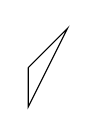
\begin{tikzpicture}[scale=0.5,baseline=1]
  \draw (0,0) -- (1,1) -- (0,-1) -- (0,0);
\end{tikzpicture}

\textbf{Trayectos cerrados}

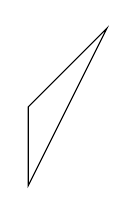
\begin{tikzpicture}
  \draw (0,0) -- (1,1) -- (0,-1) -- cycle;
\end{tikzpicture}

\textbf{Trayectos separados}

\begin{tikzpicture}
  \draw (0,0) -- (2,0) (0,1) -- (2,1);
\end{tikzpicture}

\textbf{Trayectorias conectadas por líneas horizontales y verticales}

\begin{tikzpicture}
  \draw (0,0) -| (4,3);
  \draw (0,0) |- (1,1);
\end{tikzpicture}

\textbf{Ejercicio: Hacer una letra L con ``volumen''}

\begin{tikzpicture}
  \draw (3,0) -| (0,4);
  \draw (3,1) -| (1,4);
  \draw (3,0) -- (3,1);
  \draw (0,4) -- (1,4);
\end{tikzpicture}

\section*{Trayectorias en curva}

Para utilizar curvas de Bezier se utiliza \verb |.. controls() .. ()|

\begin{tikzpicture}
  \draw (0,0) .. controls (2,2) .. (4,0) .. controls(5,-1) .. (6,0);
\end{tikzpicture}

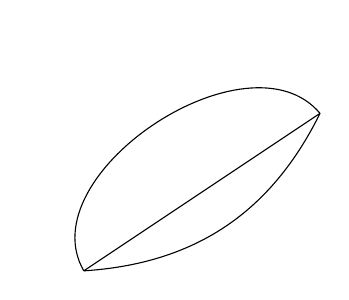
\begin{tikzpicture}
  \draw (0,0) to (3,2);
  \draw (0,0) to[out=120,in=130] (3,2);
  \draw (0,0) to[bend right] (3,2);
\end{tikzpicture}

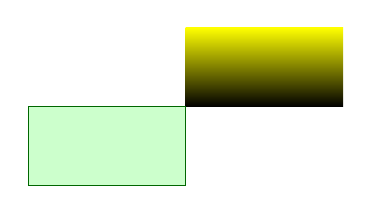
\begin{tikzpicture}
  \shade[top color=yellow, bottom color=black] (2,1) rectangle (4,2);
  \filldraw[fill=green!20!white, draw=green!40!black] (0,0) rectangle (2,1);
\end{tikzpicture}

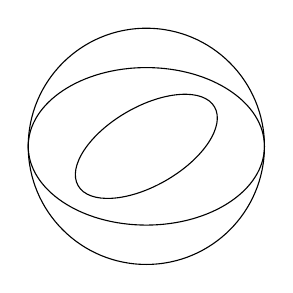
\begin{tikzpicture}
  \draw (0,0) circle [radius=1.5];
  \draw (0,0) circle [x radius=1.5cm, y radius=10mm];
  \draw (0,0) circle [x radius=1cm, y radius=5mm, rotate=30];
\end{tikzpicture}

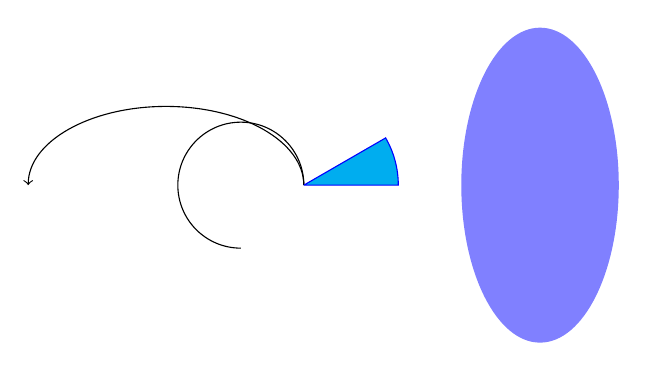
\begin{tikzpicture}
  \draw (0,0) arc (0:270:8mm);
  \draw[->] (0,0) arc (0:180:1.75cm and 1cm);
  \filldraw[fill=cyan, draw=blue] (0,0) -- (12mm,0mm) arc (0:30:12mm) -- (0,0);
  \fill[blue!50] (3,0) ellipse (1 and 2);
\end{tikzpicture}

\textbf{Ejercicio, dibujar un pacman}

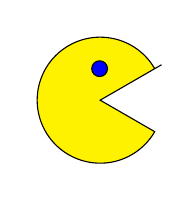
\begin{tikzpicture}
  %\filldraw[fill=yellow, draw=blue] (0,-1) -- (12mm,0mm) arc (30:300:12mm) -- (0,0);
  \filldraw[fill=yellow] (0,0) arc (30:330:8mm)  -- (30:-8mm) -- (30:1mm);
  \filldraw[fill=blue] (-7mm,0) circle[radius=1mm];
\end{tikzpicture}


\begin{tikzpicture}
  \draw[help lines] (0,0) grid (4,4);
\end{tikzpicture}

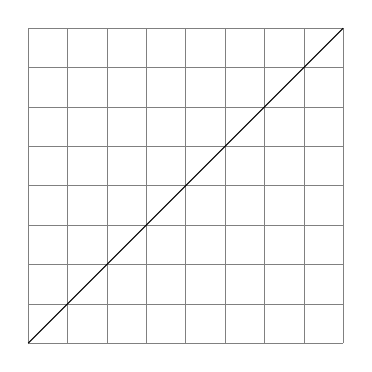
\begin{tikzpicture}
  \draw[step=0.5, gray, very thin] (0,0) grid (4,4);
  \draw[step=0.5] (0,0) -- (4,4);
\end{tikzpicture}

\section*{Funciones}

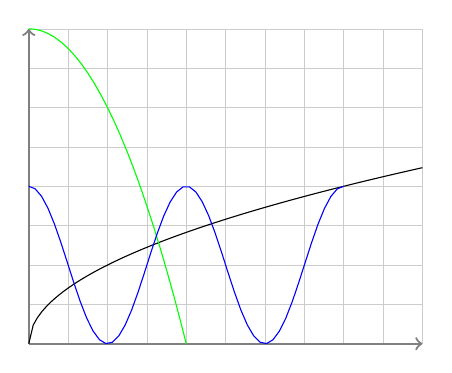
\begin{tikzpicture}
  \draw[step=0.5, gray!40, very thin] (0,0) grid (5,4);
  \draw[->, thick,gray] (0,0) -- (0,4);
  \draw[->, thick, gray] (0,0) -- (5,0);
  \draw [domain=0:5,samples=90] plot (\x, {sqrt(\x)});
  \draw [green, domain=0:2] plot (\x, {4-\x*\x});
  \draw [domain=0:4, blue,samples=50] plot (\x, {1+cos(pi*\x r)});
\end{tikzpicture}

\section*{Uso de nodos}

\begin{tikzpicture}
  \draw[dotted] (0,0) node[below]{n1} -- (1,1) node[right]{n2} -- (0,2) node[above]{n3};
\end{tikzpicture}

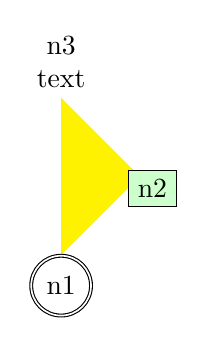
\begin{tikzpicture}
  \fill[fill=yellow] (0,0) node[below,double,circle,draw]{n1} -- 
  (1,1) node[right,fill=green!20,rectangle,draw,pos=0.85]{n2} -- 
  % Es necesario especificar la opción align para texto multilinea
  (0,2) node[align=center,above]{n3\\text};
\end{tikzpicture}

\begin{tikzpicture}
  %\path (0,0) node(x) {} (3,1) node(y) {};
  \coordinate (x) at (0,0);
  \coordinate (y) at (3,1);
  \draw (x) -- (y);
\end{tikzpicture}

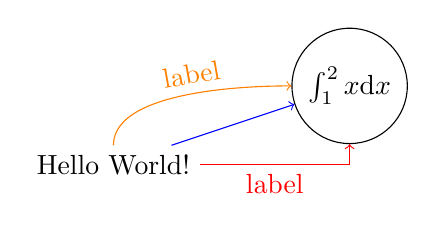
\begin{tikzpicture}
  \path (0,0) node(x) {Hello World!}
  (3,1) node[circle,draw](y) {$\int_1^2 x \mathrm d x$};
  \draw[->,blue] (x) -- (y);
  \draw[->,red] (x) -| node[near start,below] {label} (y);
  \draw[->,orange] (x) .. controls +(up:1cm) and +(left:1cm) .. 
  node[above,sloped] {label} (y);
\end{tikzpicture}

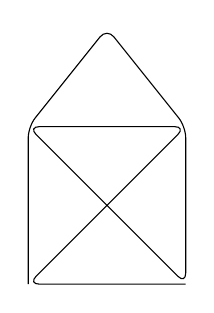
\begin{tikzpicture}
  \draw[rounded corners] (0,0) -- (0,2) -- (1,3.25) -- (2,2) -- (2,0) -- (0,2) -- (2,2) -- (0,0) -- (2,0);
\end{tikzpicture}

\textbf{Ejercicio en clase}

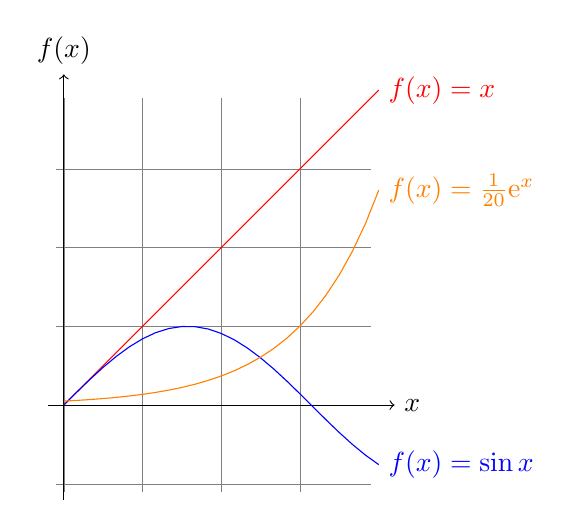
\begin{tikzpicture}[domain=0:4] 
  \draw[very thin,color=gray] (-0.1,-1.1) grid (3.9,3.9);
  \draw[->] (-0.2,0) -- (4.2,0) node[right] {$x$}; 
  \draw[->] (0,-1.2) -- (0,4.2) node[above] {$f(x)$};
  \draw[color=red]    plot (\x,\x)             node[right] {$f(x) =x$}; 
  \draw[color=blue]   plot (\x,{sin(\x r)})    node[right] {$f(x) = \sin x$}; 
  \draw[color=orange] plot (\x,{0.05*exp(\x)}) node[right] {$f(x) = \frac{1}{20} \mathrm e^x$};
\end{tikzpicture}

\textbf{Ejercicio en clase}

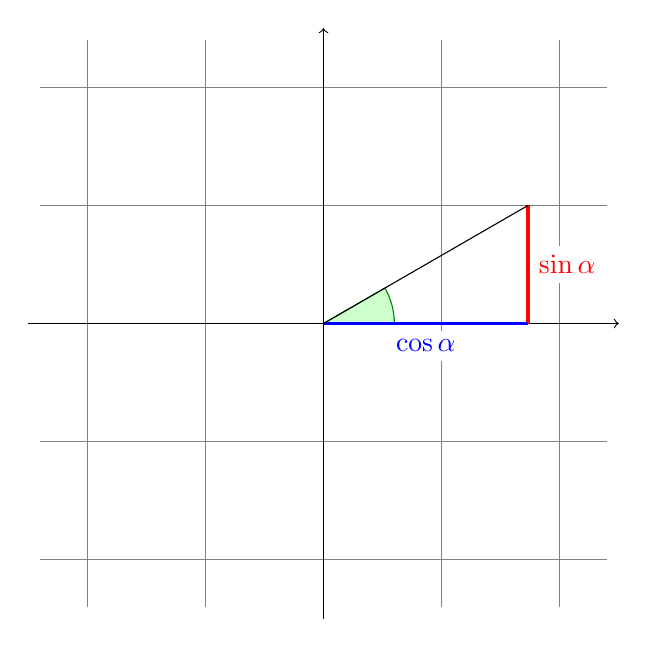
\begin{tikzpicture}[scale=3]
\draw[step=.5cm, gray, very thin] (-1.2,-1.2) grid (1.2,1.2); 
\filldraw[fill=green!20,draw=green!50!black] (0,0) -- (3mm,0mm) arc (0:30:3mm) -- cycle; 
\draw[->] (-1.25,0) -- (1.25,0) coordinate (x axis);
\draw[->] (0,-1.25) -- (0,1.25) coordinate (y axis);
\draw[very thick,red] (30:1cm) -- node[right,fill=white] {$\sin \alpha$} (30:1cm |- x axis);
\draw[very thick,blue] (30:1cm |- x axis) -- node[below=2pt,fill=white] {$\cos \alpha$} (0,0);
\draw (0,0) -- (30:1cm);
\end{tikzpicture}


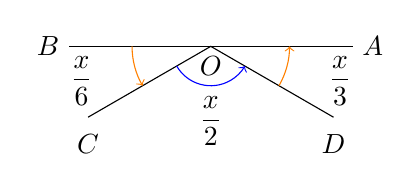
\begin{tikzpicture}[scale=0.6]
  \draw
  (30:-3) coordinate (c) node[below=1mm] {$C$} -- 
  (0,0) coordinate (o) node[below] {$O$} -- 
  (150:-3) coordinate (d) node[below=1mm ] {$D$}
  pic["$\dfrac{x}{2}$",draw=blue,->,angle eccentricity=1.9,angle radius=5mm] 
    {angle=c--o--d};
  \draw (o) -- (3,0) coordinate (a) node[right] {$A$};
  \draw (o) -- (-3,0) coordinate (b) node[left] {$B$};
  \pic["$\dfrac{x}{6}$",draw=orange,->,angle eccentricity=1.7,angle radius=1cm] 
    {angle=b--o--c};
  \pic["$\dfrac{x}{3}$",draw=orange,->,angle eccentricity=1.7,angle radius=1cm] 
    {angle=d--o--a};
\end{tikzpicture}

\end{multicols}

\end{document}
